\documentclass[tikz,border=2pt]{standalone}
\usepackage{pgfplots}
\usetikzlibrary{intersections}
\usetikzlibrary{positioning}
\usetikzlibrary{calc}
\usepgfplotslibrary{fillbetween}
\begin{document}

\tikzset{%
  dots/.style args={#1per #2}{%
    line cap=round,
    dash pattern=on 0 off #2/#1
  }
}

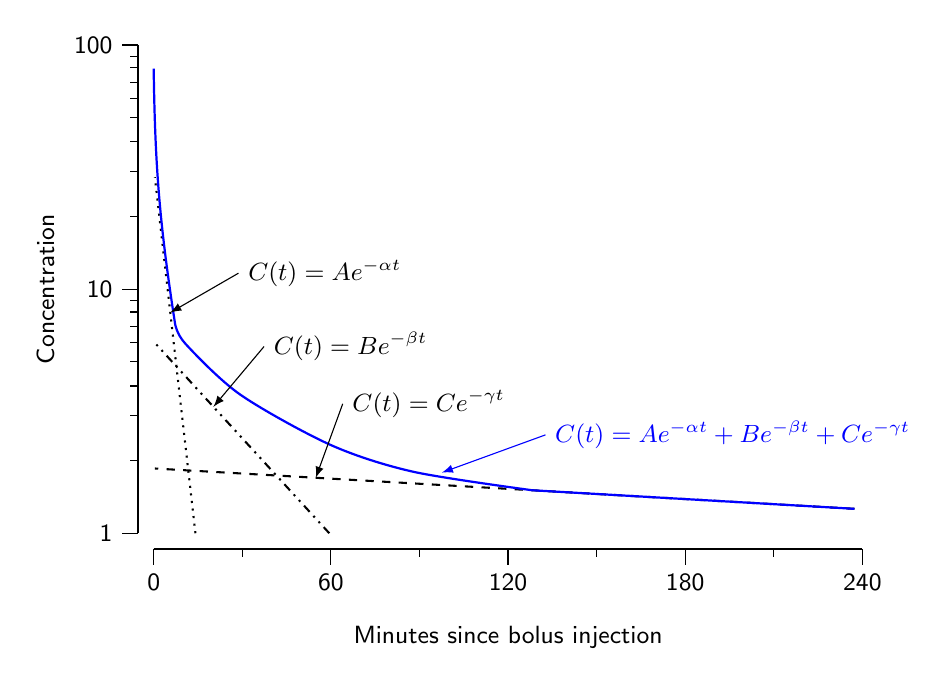
\begin{tikzpicture}[font=\sffamily\small]
\draw[line width=0.5pt](0,0)--(9,0);
\foreach \x/\y in {0/0,2.25/60,4.5/120,6.75/180,9/240}
\draw[](\x,0)--(\x,-0.2)node[below](X\y){\y};

\foreach \x in {1.125,3.375,5.625,7.875}
\draw[](\x,0)--(\x,-0.1)node[below](X\x){};
\node[below=2mm of X120]{Minutes since bolus injection};
%%y
\draw[line width=0.5pt](-0.2,0.2)--(-0.2,6.4);
\foreach \x/\y in {0.2/1,3.3/10,6.4/100}
\draw[](-0.2,\x)--(-0.4,\x)node[left](Y\y){\y};
\foreach \x in {1.12,1.69,2.07,2.38,2.62,2.82,3.01,3.16,%
4.22,4.79,5.17,5.48,5.72,5.92,6.11,6.26}
\draw[](-0.2,\x)--(-0.3,\x)node[left](Y\x){};
\node[left=4mm of Y10,rotate=90,anchor=center]{Concentration};

\coordinate(D)at(8.9,0.51);
\coordinate(G)at(0,6.1);

\draw[line width=0.75pt, dashed](D)--++(176.7:8.9)coordinate(DD);
\draw[line width=0.75pt, dotted](0.53,0.2)
coordinate(A)--++(96.5:4.55)coordinate(AA);
\draw[line width=0.75pt,dash dot dot](2.23,0.2)
coordinate(B)--++(132.5:3.25)coordinate(BB);
\draw[blue,thick](D)--++(176.7:4.1)coordinate(D1)
(0.27,2.87)coordinate(D2)to[bend left=4](G);
\draw [blue,thick]
plot [smooth] coordinates {(D1)(3.3,0.98) (2.25,1.32)(1.1,1.96) 
(0.4,2.61)(D2)};

%Arrows
 \draw[latex-]($(A)!0.62!(AA)$)--++(30:1)node[right]{$C(t)=Ae^{-\alpha t}$};
 \draw[latex-]($(B)!0.67!(BB)$)--++(50:1)node[right]{$C(t)=Be^{-\beta t}$};
  \draw[latex-]($(D)!0.77!(DD)$)--++(70:1)node[right]{$C(t)=Ce^{-\gamma t}$};
  \draw[latex-,shorten <=-4mm, blue]($(D1)!0.17!(D2)$)--++(20:1)node[right]{$C(t)=
 Ae^{-\alpha t}+Be^{-\beta t}+ Ce^{-\gamma t}$}; 
\end{tikzpicture}
\end{document}
